\documentclass[12pt,a4paper]{article}
\usepackage{graphicx}
\usepackage[utf8]{inputenc}
\usepackage[T5]{fontenc}
\usepackage[top=2.5cm, bottom=2.5cm, left=2.5cm, right=2cm]{geometry}
\usepackage{fancyhdr}
\usepackage{titlesec}
\usepackage{array}
\usepackage{setspace}
\usepackage{tikz}
\usetikzlibrary{positioning,arrows.meta,fit}
\usepackage{hyperref}
\usepackage{tocloft}
\usepackage{float}
\usepackage{makecell}
\usepackage{tabularx}
\usepackage{longtable}
\usepackage{ragged2e}
\usepackage{enumitem}
\usepackage{indentfirst}
\usepackage{xcolor}

\hypersetup{colorlinks=true, linkcolor=blue, urlcolor=blue, citecolor=blue}
\pagenumbering{arabic}
\pagestyle{fancy}
\fancyhf{}
\fancyhead[L]{VisionDriveAI Specification}
\fancyhead[C]{AIoT Project}
\fancyhead[R]{VisionDriveAI}
\renewcommand{\footrulewidth}{0.4pt}
\fancyfoot[L]{University of Science}
\fancyfoot[C]{Faculty of Information Technology}
\fancyfoot[R]{Page \thepage}

\renewcommand{\arraystretch}{1.25}
\setlength{\parindent}{1.2cm}
\setlength{\parskip}{0.2cm}
\newcolumntype{L}{>{\raggedright\arraybackslash}X}
\newcolumntype{P}[1]{>{\raggedright\arraybackslash}p{#1}}

\titleformat{\section}{\Large\bfseries}{\thesection}{1em}{}
\titleformat{\subsection}{\large\bfseries}{\thesubsection}{1em}{}
\titleformat{\subsubsection}{\normalsize\bfseries}{\thesubsubsection}{1em}{}

\begin{document}

\thispagestyle{empty}

\begin{tikzpicture}[remember picture, overlay]
  \draw[blue, line width=3pt] ([xshift=1cm,yshift=-1cm]current page.north west)
    rectangle ([xshift=-1cm,yshift=1cm]current page.south east);
  \draw[blue, line width=3pt] ([xshift=1cm,yshift=-1cm]current page.north west) -- ++(1cm,0);
  \draw[blue, line width=3pt] ([xshift=1cm,yshift=-1cm]current page.north west) -- ++(0,-1cm);
  \draw[blue, line width=3pt] ([xshift=-1cm,yshift=1cm]current page.south east) -- ++(-1cm,0);
  \draw[blue, line width=3pt] ([xshift=-1cm,yshift=1cm]current page.south east) -- ++(0,1cm);
\end{tikzpicture}

\begin{center}
    \vspace{-1cm}
    \textbf{\large VIETNAM NATIONAL UNIVERSITY, HO CHI MINH CITY} \\ [0.3cm]
    \textbf{\Large UNIVERSITY OF SCIENCE} \\ [0.3cm]
    \textit{Faculty of Information Technology} \\
    \vspace{1.2cm}

    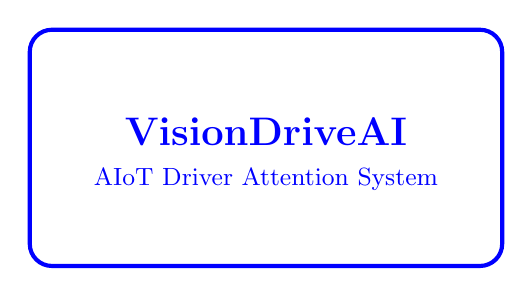
\begin{tikzpicture}
      \draw[blue, line width=1.5pt, rounded corners=8pt] (0,0) rectangle (6,3);
      \node[blue, font=\Large\bfseries] at (3,1.7) {VisionDriveAI};
      \node[blue, font=\small] at (3,1.1) {AIoT Driver Attention System};
    \end{tikzpicture}
    \vspace{0.8cm}

    {\LARGE \textbf{VISIONDRIVEAI SPECIFICATION}} \\[0.5cm]
    {\Large \textbf{AIOT DISTRACTION DETECTION SYSTEM FOR URBAN MOTORBIKES}} \\[0.7cm]
    {\Large Course: Introduction to Smart Device Programming} \\
    \vspace{0.8cm}

    \begin{flushleft}
        \textbf{CLASS:} 23CLC02 \\[0.4cm]
        \textbf{PROJECT:} VisionDriveAI - Tập trung hơn, lái xe an toàn hơn. \\[0.5cm]
        \textbf{MEMBER INFORMATION:}
    \end{flushleft}

    \small
    \begin{tabularx}{\textwidth}{|c|P{3cm}|P{1.8cm}|P{2.2cm}|X|}
    \hline
    \textbf{STT} & \textbf{Member} & \textbf{Student ID} & \textbf{Phone Number} & \textbf{Email} \\
    \hline
    1 & Trần Hải Đức & 23127173 & 0916821170 & thduc23@clc.fitus.edu.vn \\
    \hline
    2 & Nguyễn Trọng Tài & 23127008 & 0377425510 & nttai23@clc.fitus.edu.vn \\
    \hline
    3 & Nguyễn Công Chiến & 23127331 & 0369314655 & ncchien23@clc.fitus.edu.vn \\
    \hline
    4 & Nguyễn Tấn Thắng & 23127259 & 0396177323 & ntthang23@clc.fitus.edu.vn \\
    \hline
    \end{tabularx}
    \normalsize

    \vfill
    \textit{TP.HCM, May 26, 2026.}
\end{center}

\newpage
\tableofcontents
\newpage

\section{Background}

\subsection{Product Overview}

VisionDriveAI là một hệ thống AIoT hỗ trợ phát hiện mất tập trung cho người lái xe máy trong môi trường nội đô. Sản phẩm được định hướng như một thiết bị edge nhỏ gọn gắn trên xe, kết hợp camera, cảm biến chuyển động và hệ thống cảnh báo tức thời để giúp người lái nhận biết sớm các hành vi nguy hiểm như ngủ gật, nhìn lạc hướng, cầm điện thoại hoặc điều khiển xe thiếu ổn định.

Trong bối cảnh giao thông đô thị Việt Nam, xe máy là phương tiện di chuyển phổ biến. Tuy nhiên, các tình huống mất tập trung khi lái xe vẫn có thể dẫn đến va chạm, xử lý chậm hoặc tạo nguy hiểm cho người đi đường. VisionDriveAI giải quyết vấn đề này bằng cách xử lý dữ liệu trực tiếp trên edge device thay vì phụ thuộc hoàn toàn vào cloud.

\begin{center}
\textbf{VisionDriveAI - Tập trung hơn, lái xe an toàn hơn.}
\end{center}

\subsection{Motivation}

Động lực phát triển VisionDriveAI xuất phát từ nhu cầu tăng cường an toàn cho người lái xe máy trong môi trường đô thị. Nhiều giải pháp hỗ trợ lái xe an toàn hiện nay tập trung vào ô tô, trong khi xe máy vẫn thiếu các thiết bị nhỏ gọn, chi phí hợp lý và phù hợp với điều kiện sử dụng hằng ngày.

VisionDriveAI tận dụng xu hướng Edge AI và AIoT: dữ liệu được xử lý ngay trên thiết bị để giảm độ trễ, hạn chế phụ thuộc Internet liên tục và bảo vệ quyền riêng tư tốt hơn. Việc kết hợp Computer Vision với dữ liệu IMU giúp hệ thống phát hiện hành vi nguy hiểm đáng tin cậy hơn.

\subsection{Intended Audience}

\begin{itemize}
    \item Người lái xe máy thường xuyên di chuyển trong nội đô.
    \item Sinh viên và nhân viên văn phòng đi lại bằng xe máy hằng ngày.
    \item Tài xế giao hàng, tài xế công nghệ hoặc người chạy xe nhiều giờ liên tục.
    \item Gia đình muốn theo dõi và nhắc nhở thói quen lái xe an toàn của người thân.
    \item Đội xe nhỏ hoặc đơn vị vận hành muốn có dữ liệu an toàn theo hành trình.
\end{itemize}

\subsection{VisionDriveAI Advantages}

\begin{itemize}
    \item Tập trung vào người lái xe máy nội đô, không phải ô tô.
    \item Xử lý trực tiếp trên edge device, giảm phụ thuộc Internet liên tục.
    \item Kết hợp camera và IMU để tăng độ tin cậy.
    \item Cảnh báo đa tầng bằng rung, còi và LED.
    \item Có app mobile để ghi log, gửi thông báo và phân tích thói quen lái xe.
    \item Chi phí prototype tương đối thấp, khoảng 375,000 VND.
\end{itemize}

\newpage
\section{Architecture and Hardware}

\subsection{Architecture}

VisionDriveAI được thiết kế theo mô hình AIoT gồm ba lớp chính: Edge Device, Mobile App và Server. Edge Device xử lý camera, IMU và cảnh báo tại chỗ. Mobile App nhận log hành trình, thông báo realtime và hiển thị phân tích. Server lưu trữ dữ liệu, phân tích pattern dài hạn và hỗ trợ cá nhân hóa mô hình.

\subsubsection{Architecture Diagram}

\begin{figure}[H]
\centering
\begin{tikzpicture}[
    node distance=1.3cm,
    box/.style={draw, rounded corners, minimum width=3.2cm, minimum height=0.85cm, align=center},
    smallbox/.style={draw, rounded corners, minimum width=2.8cm, minimum height=0.7cm, align=center, font=\small},
    arrow/.style={-{Latex}, thick}
]
    \node[box] (rider) {Người lái};
    \node[box, right=2cm of rider] (edge) {VisionDriveAI\\Edge Device};
    \node[smallbox, above=0.9cm of edge] (cam) {ESP32-CAM};
    \node[smallbox, below=0.9cm of edge] (imu) {MPU-6050 IMU};
    \node[box, right=2.3cm of edge] (app) {Mobile App};
    \node[box, right=2.3cm of app] (server) {VisionDriveAI\\Server};
    \node[smallbox, below=0.9cm of app] (alert) {Vibration\\Buzzer\\LED};

    \draw[arrow] (rider) -- (edge);
    \draw[arrow] (cam) -- (edge);
    \draw[arrow] (imu) -- (edge);
    \draw[arrow] (edge) -- (alert);
    \draw[arrow] (alert) -- (rider);
    \draw[<->, thick] (edge) -- (app);
    \draw[<->, thick] (app) -- (server);
\end{tikzpicture}
\caption{VisionDriveAI Edge-Mobile-Server Architecture}
\end{figure}

\subsubsection{Data Flow}

\begin{longtable}{|c|P{12.5cm}|}
\hline
\textbf{Step} & \textbf{Description} \\
\hline
1 & Camera ghi nhận khuôn mặt, hướng nhìn và tư thế tay của người lái. \\
\hline
2 & MPU-6050 ghi nhận chuyển động tay lái, lắc lư, phanh gấp hoặc mất ổn định. \\
\hline
3 & ESP32-S3 xử lý dữ liệu hình ảnh và IMU bằng logic Edge AI / Sensor Fusion. \\
\hline
4 & Khi phát hiện rủi ro, hệ thống kích hoạt cảnh báo rung, buzzer hoặc LED. \\
\hline
5 & Sự kiện được ghi log với timestamp, loại hành vi và metadata liên quan. \\
\hline
6 & Mobile App nhận thông báo và hiển thị lịch sử hành trình. \\
\hline
7 & Server tổng hợp dữ liệu dài hạn để phân tích pattern và cá nhân hóa mô hình. \\
\hline
\caption{VisionDriveAI Data Flow}
\end{longtable}

\subsection{Hardware}

\begin{longtable}{|P{3cm}|c|P{2.2cm}|P{2cm}|P{4.2cm}|P{2.3cm}|}
\hline
\textbf{Component} & \textbf{Qty} & \textbf{Availability} & \textbf{Interface} & \textbf{Purpose} & \textbf{Estimated Price} \\
\hline
ESP32-S3 DevKitC-1 (N8R8 hoặc N16R8) & 1 & Mua thêm & Wi-Fi, BLE, SPI, I2C & Edge AI inference, Sensor Fusion và upload log lên app/server. & 150,000 - 220,000 VND \\
\hline
ESP32-CAM (OV2640 2MP) Ai-Thinker & 1 & Mua thêm & UART / Wi-Fi LAN & Camera nhận diện khuôn mặt, hướng nhìn, tay và điện thoại. & 225,000 VND \\
\hline
MPU-6050 GY-521 (Accel + Gyro 6DOF) & 1 & Mua thêm & I2C & Phân tích chuyển động tay lái, loại false positive khi xe dừng và phát hiện phanh gấp. & 30,000 VND \\
\hline
Vibration Motor DC coin 10mm & 1 & Mua thêm & GPIO PWM qua NPN & Cảnh báo mức 1 bằng rung tay lái. & 20,000 VND \\
\hline
Buzzer passive 5V & 1 & Mua thêm & GPIO PWM & Cảnh báo mức 2 bằng beep ngắn và mức 3 bằng còi liên tục. & 8,000 VND \\
\hline
LED RGB common cathode & 1 & Mua thêm & GPIO PWM x3 & Cảnh báo mức 3 bằng LED đỏ nháy. & 5,000 VND \\
\hline
Pin LiPo 3.7V 2000mAh + TP4056 + MT3608 & 1 & Mua thêm & Power & Nguồn độc lập cho toàn hệ thống. & 80,000 VND \\
\hline
Transistor NPN 2N2222/BC547 & 3 & Mua thêm & Driver & Driver cho motor rung và buzzer, bảo vệ GPIO ESP32. & 5,000 VND \\
\hline
INMP441 Microphone & 1 & Có sẵn, tùy chọn & I2S & Đo noise level môi trường nếu mở rộng tính năng. & 40,000 - 55,000 VND \\
\hline
\caption{Hardware Components and Estimated Cost}
\end{longtable}

\begin{longtable}{|P{5cm}|P{7cm}|}
\hline
\textbf{Cost Type} & \textbf{Estimated Range} \\
\hline
Required additional components & Approximately 518,000 VND \\
\hline
\caption{Estimated Total Cost}
\end{longtable}

\newpage
\section{Objectives}

\subsection{Overview}

VisionDriveAI được phát triển với mục tiêu trở thành một hệ thống hỗ trợ an toàn cho người lái xe máy nội đô bằng cách phát hiện hành vi mất tập trung, cảnh báo tức thời và phân tích thói quen lái xe dài hạn.

\subsection{Overall Use Case Diagram}

\begin{figure}[H]
\centering
\begin{tikzpicture}[
    node distance=1.1cm,
    actor/.style={draw, ellipse, minimum width=2.6cm, minimum height=0.8cm},
    usecase/.style={draw, rounded corners, minimum width=5.4cm, minimum height=0.72cm, align=center, font=\small},
    arrow/.style={-{Latex}, thick}
]
    \node[actor] (user) {Người lái};
    \node[usecase, right=3.2cm of user, yshift=2.5cm] (uc1) {Ngủ gật và nhìn lạc hướng};
    \node[usecase, below=0.45cm of uc1] (uc2) {Cầm điện thoại khi lái};
    \node[usecase, below=0.45cm of uc2] (uc3) {Cảnh báo leo thang 3 mức};
    \node[usecase, below=0.45cm of uc3] (uc4) {Realtime notification và AI pattern};
    \node[usecase, below=0.45cm of uc4] (uc5) {Safety Score theo chuyến};
    \node[usecase, below=0.45cm of uc5] (uc6) {Cá nhân hóa mô hình};

    \foreach \x in {uc1,uc2,uc3,uc4,uc5,uc6} \draw[arrow] (user) -- (\x);
\end{tikzpicture}
\caption{Overall VisionDriveAI Use Cases}
\end{figure}

\subsection{Objective 1: Real-Time Distraction Detection}

Objective đầu tiên của VisionDriveAI là phát hiện các hành vi nguy hiểm ngay khi chúng xảy ra. Hệ thống sử dụng Computer Vision chạy trên edge kết hợp dữ liệu IMU để nhận diện các tình huống có thể làm giảm khả năng phản ứng của người lái.

\subsubsection{Use Case 1: Drowsiness and Gaze Deviation Detection}

ESP32-CAM hướng vào khuôn mặt người lái để phát hiện mắt nhắm quá lâu, đầu gật xuống hoặc ánh mắt nhìn sang hướng khác trong thời gian liên tục.

\begin{longtable}{|P{3.5cm}|P{11cm}|}
\hline
\textbf{Actor} & Rider \\
\hline
\textbf{Goal} & Phát hiện sớm tình trạng buồn ngủ hoặc nhìn lạc hướng khi lái xe. \\
\hline
\textbf{Preconditions} & Camera đã được lắp đúng hướng và Edge Device đang hoạt động. \\
\hline
\textbf{Main Flow} & Camera ghi nhận khuôn mặt, Edge AI phân tích mắt/hướng nhìn, hệ thống xác định rủi ro và gửi tín hiệu cảnh báo. \\
\hline
\textbf{Expected Result} & Người lái được cảnh báo trước khi tình huống mất tập trung kéo dài. \\
\hline
\textbf{AI Involvement} & Yes \\
\hline
\caption{Drowsiness and Gaze Deviation Use Case}
\end{longtable}

\subsubsection{Use Case 2: Phone Holding Detection}

Camera góc rộng và mô hình nhận diện nhẹ phát hiện tư thế tay có dấu hiệu cầm điện thoại. Dữ liệu IMU hỗ trợ phân biệt tình huống xe đang dừng và xe đang di chuyển.

\begin{longtable}{|P{3.5cm}|P{11cm}|}
\hline
\textbf{Actor} & Rider \\
\hline
\textbf{Goal} & Phát hiện hành vi dùng điện thoại trong lúc lái xe. \\
\hline
\textbf{Preconditions} & Camera và IMU đang hoạt động. \\
\hline
\textbf{Main Flow} & Camera phát hiện tư thế tay, IMU xác nhận trạng thái di chuyển, hệ thống đánh giá rủi ro và kích hoạt cảnh báo. \\
\hline
\textbf{Expected Result} & Người lái được nhắc nhở khi có hành vi cầm điện thoại nguy hiểm. \\
\hline
\textbf{AI Involvement} & Yes \\
\hline
\caption{Phone Holding Detection Use Case}
\end{longtable}

\subsection{Objective 2: Multi-Level Alert and Immediate Feedback}

Objective thứ hai tập trung vào việc phản hồi nhanh nhưng không gây hoảng loạn. VisionDriveAI sử dụng cảnh báo leo thang theo thời gian và mức độ rủi ro.

\subsubsection{Use Case 3: Three-Level Escalation Alert}

\begin{longtable}{|P{3.5cm}|P{11cm}|}
\hline
\textbf{Actor} & Rider \\
\hline
\textbf{Goal} & Cảnh báo người lái theo mức độ nguy hiểm. \\
\hline
\textbf{Preconditions} & Edge Device đã phát hiện hành vi rủi ro. \\
\hline
\textbf{Main Flow} & Rủi ro bắt đầu, kích hoạt rung nhẹ, nếu kéo dài tăng lên rung mạnh và beep, nếu tiếp tục nguy hiểm tăng lên còi liên tục và LED đỏ. \\
\hline
\textbf{Expected Result} & Người lái được nhắc nhở kịp thời mà không bị cảnh báo quá đột ngột. \\
\hline
\textbf{AI Involvement} & No direct AI \\
\hline
\caption{Three-Level Alert Use Case}
\end{longtable}

\subsubsection{Use Case 4: Realtime Notification and AI Pattern Analysis}

\begin{longtable}{|P{3.5cm}|P{11cm}|}
\hline
\textbf{Actor} & Rider, Family Member, Fleet Manager \\
\hline
\textbf{Goal} & Theo dõi sự kiện mất tập trung và phân tích pattern dài hạn. \\
\hline
\textbf{Preconditions} & App và Server đã được cấu hình. \\
\hline
\textbf{Main Flow} & Edge ghi log, App nhận thông báo, Server lưu dữ liệu, AI phân tích pattern và hệ thống cập nhật độ nhạy khi cần. \\
\hline
\textbf{Expected Result} & Người dùng hiểu được thời điểm hoặc điều kiện thường gây mất tập trung. \\
\hline
\textbf{AI Involvement} & Yes \\
\hline
\caption{Realtime Notification and AI Pattern Use Case}
\end{longtable}

\subsection{Objective 3: Trip Analytics and Personalization}

Objective thứ ba giúp VisionDriveAI chuyển từ một thiết bị cảnh báo tức thời thành một hệ thống cải thiện hành vi lái xe dài hạn.

\subsubsection{Use Case 5: Trip Safety Score}

\begin{longtable}{|P{3.5cm}|P{11cm}|}
\hline
\textbf{Actor} & Rider \\
\hline
\textbf{Goal} & Xem mức độ an toàn sau mỗi chuyến đi. \\
\hline
\textbf{Preconditions} & Hành trình đã được ghi log. \\
\hline
\textbf{Main Flow} & App tổng hợp dữ liệu, tính Safety Score, hiển thị dashboard và xu hướng. \\
\hline
\textbf{Expected Result} & Người lái hiểu được chất lượng lái xe và các điểm cần cải thiện. \\
\hline
\textbf{AI Involvement} & No direct AI \\
\hline
\caption{Trip Safety Score Use Case}
\end{longtable}

\subsubsection{Use Case 6: Personalized Driver Model}

\begin{longtable}{|P{3.5cm}|P{11cm}|}
\hline
\textbf{Actor} & Rider \\
\hline
\textbf{Goal} & Cá nhân hóa mô hình phát hiện để giảm cảnh báo nhầm. \\
\hline
\textbf{Preconditions} & Hệ thống đã có đủ dữ liệu lịch sử. \\
\hline
\textbf{Main Flow} & Server phân tích dữ liệu, xác định baseline, cập nhật ngưỡng/mô hình và Edge áp dụng cấu hình cá nhân hóa. \\
\hline
\textbf{Expected Result} & Hệ thống cảnh báo chính xác hơn theo từng người lái. \\
\hline
\textbf{AI Involvement} & Yes \\
\hline
\caption{Personalized Driver Model Use Case}
\end{longtable}

\subsection{Use Case Summary}

\begin{longtable}{|P{3.2cm}|P{4cm}|c|P{5.2cm}|}
\hline
\textbf{Objective} & \textbf{Use Case} & \textbf{AI} & \textbf{Expected Result} \\
\hline
Real-time detection & Ngủ gật và nhìn lạc hướng & Yes & Người lái được cảnh báo kịp thời. \\
\hline
Real-time detection & Cầm điện thoại khi lái & Yes & Giảm rủi ro do dùng điện thoại khi lái xe. \\
\hline
Alert and feedback & Cảnh báo leo thang 3 mức & No & Cảnh báo hiệu quả nhưng ít gây hoảng loạn. \\
\hline
Alert and feedback & Realtime notification và AI pattern & Yes & Người dùng nắm được thời điểm/khu vực rủi ro. \\
\hline
Analytics and personalization & Safety Score theo chuyến & No & Người lái có insight cải thiện thói quen. \\
\hline
Analytics and personalization & Cá nhân hóa mô hình & Yes & Giảm false positive và tăng độ chính xác. \\
\hline
\caption{Use Case Summary}
\end{longtable}

\newpage
\section{User Manual}

\subsection{Overview}

Tài liệu này hướng dẫn người dùng thiết lập và sử dụng VisionDriveAI. Hệ thống gồm Edge Device gắn trên xe máy, camera, cảm biến IMU, cụm cảnh báo rung/còi/LED và ứng dụng di động để theo dõi hành trình.

\subsection{Device Setup}

\begin{enumerate}
    \item Gắn Edge Device ở vị trí chắc chắn trên xe máy.
    \item Đặt ESP32-CAM hướng về khuôn mặt và phần tay lái của người lái.
    \item Gắn vibration motor gần khu vực ghi đông.
    \item Đặt buzzer và LED ở vị trí dễ nghe, dễ nhìn nhưng không che khuất tầm nhìn.
    \item Bật Edge Device và chờ trạng thái sẵn sàng.
\end{enumerate}

\subsection{Mobile App Connection}

\begin{enumerate}
    \item Bật Bluetooth hoặc Wi-Fi trên điện thoại.
    \item Mở ứng dụng VisionDriveAI.
    \item Chọn Pair New Device.
    \item Chọn thiết bị VisionDriveAI trong danh sách.
    \item Xác nhận kết nối và kiểm tra trạng thái camera, IMU và pin.
\end{enumerate}

\subsection{Starting a Ride}

\begin{enumerate}
    \item Bật Edge Device trước khi bắt đầu di chuyển.
    \item Kiểm tra camera không bị che khuất.
    \item Kiểm tra thiết bị có nhận được dữ liệu IMU.
    \item Mở app và nhấn Start Trip nếu muốn ghi log hành trình.
    \item Bắt đầu lái xe như bình thường.
\end{enumerate}

\subsection{Alert System}

\begin{longtable}{|P{2.5cm}|P{5cm}|P{6.5cm}|}
\hline
\textbf{Level} & \textbf{Condition} & \textbf{Alert} \\
\hline
Level 1 & Rủi ro mới xuất hiện & Rung nhẹ ở ghi đông. \\
\hline
Level 2 & Rủi ro kéo dài & Rung mạnh và buzzer beep ngắn. \\
\hline
Level 3 & Rủi ro nghiêm trọng hoặc kéo dài hơn & Còi liên tục và LED đỏ nháy. \\
\hline
\caption{Alert System}
\end{longtable}

\subsection{Safety Score}

Sau mỗi chuyến đi, app tổng hợp số lần mất tập trung, tổng thời gian mắt nhắm hoặc nhìn lạc hướng, số lần cầm điện thoại, số lần phanh gấp và tần suất cảnh báo để hiển thị Safety Score từ 0 đến 100.

\subsection{Notes}

\begin{itemize}
    \item Không điều chỉnh thiết bị khi đang lái xe.
    \item Đảm bảo camera không che khuất tầm nhìn và không vi phạm quyền riêng tư của người khác.
    \item Kiểm tra pin trước mỗi chuyến đi.
    \item Cảnh báo của VisionDriveAI chỉ là công cụ hỗ trợ, không thay thế trách nhiệm quan sát và điều khiển xe an toàn.
\end{itemize}

\newpage
\section{Conclusion}

\subsection{Project Summary}

VisionDriveAI được định hướng như một hệ thống AIoT hỗ trợ an toàn cho người lái xe máy trong môi trường nội đô. Sản phẩm kết hợp Computer Vision, IMU, Edge AI, cảnh báo đa tầng và ứng dụng di động để phát hiện mất tập trung, phản hồi tức thời và phân tích thói quen lái xe dài hạn.

\subsection{Business and User Value}

\begin{itemize}
    \item \textbf{Safety value:} hỗ trợ người lái nhận biết sớm tình huống mất tập trung.
    \item \textbf{Behavior value:} giúp người dùng hiểu rõ thói quen lái xe và cải thiện theo dữ liệu.
    \item \textbf{Scalability value:} có thể mở rộng cho gia đình, tài xế giao hàng, đội xe nhỏ hoặc nghiên cứu AIoT.
\end{itemize}

\subsection{Limitations}

\begin{itemize}
    \item Camera có thể bị ảnh hưởng bởi ánh sáng yếu, mưa hoặc vị trí lắp đặt không ổn định.
    \item Edge AI trên vi điều khiển có giới hạn về hiệu năng và bộ nhớ.
    \item Dữ liệu cá nhân và hình ảnh cần được xử lý cẩn thận để bảo vệ quyền riêng tư.
    \item Hệ thống cần thử nghiệm thực tế nhiều hơn để hiệu chỉnh ngưỡng cảnh báo.
\end{itemize}

\subsection{Future Development}

\begin{itemize}
    \item Tối ưu mô hình Edge AI để chạy ổn định hơn trên thiết bị nhúng.
    \item Thiết kế vỏ chống rung, chống bụi và phù hợp với xe máy.
    \item Bổ sung cơ chế làm mờ ảnh hoặc chỉ lưu metadata.
    \item Cải thiện thuật toán Sensor Fusion giữa camera và IMU.
    \item Mở rộng dashboard cho người thân hoặc đội xe.
    \item Tích hợp bản đồ để xác định đoạn đường thường xảy ra mất tập trung.
\end{itemize}

\subsection{Final Conclusion}

VisionDriveAI là một dự án có tính ứng dụng cao trong bối cảnh xe máy là phương tiện phổ biến tại Việt Nam. Bằng cách đưa Computer Vision và Sensor Fusion lên edge device, hệ thống có thể hỗ trợ người lái ngay tại thời điểm nguy hiểm thay vì chỉ ghi nhận dữ liệu sau sự kiện.

\begin{center}
\textbf{VisionDriveAI - Tập trung hơn, lái xe an toàn hơn.}
\end{center}

\newpage
\section{Appendix and Reference}

\subsection{Key Terms}

\begin{longtable}{|P{3.2cm}|P{11.2cm}|}
\hline
\textbf{Term} & \textbf{Description} \\
\hline
VisionDriveAI & Hệ thống AIoT phát hiện mất tập trung cho người lái xe máy nội đô. \\
\hline
Edge Device & Thiết bị gắn trên xe, xử lý camera, IMU và cảnh báo tại chỗ. \\
\hline
Computer Vision & Kỹ thuật xử lý hình ảnh để nhận diện khuôn mặt, hướng nhìn hoặc tư thế tay. \\
\hline
Sensor Fusion & Kết hợp dữ liệu từ nhiều cảm biến để tăng độ tin cậy khi ra quyết định. \\
\hline
Safety Score & Điểm đánh giá mức độ an toàn của chuyến đi, thường trong thang 0-100. \\
\hline
\caption{Key Terms}
\end{longtable}

\begin{thebibliography}{9}
\bibitem{esp32s3}
ESP32-S3 Series, Espressif Systems. \url{https://www.espressif.com/en/products/socs/esp32-s3}

\bibitem{esp32cam}
ESP32 Camera Driver, Espressif Component Registry. \url{https://components.espressif.com/components/espressif/esp32-camera}

\bibitem{mpu6050}
MPU-6050 Six-Axis MotionTracking Device, TDK InvenSense. \url{https://invensense.tdk.com/products/motion-tracking/6-axis/mpu-6050/}

\bibitem{mediapipe}
MediaPipe Face Landmarker, Google AI. \url{https://ai.google.dev/edge/mediapipe/solutions/vision/face_landmarker}

\bibitem{mobilenet}
MobileNets, Google Research. \url{https://research.google/pubs/mobilenets-efficient-convolutional-neural-networks-for-mobile-vision-applications/}

\bibitem{edgeai}
Edge AI overview, IBM. \url{https://www.ibm.com/think/topics/edge-ai}
\end{thebibliography}

\end{document}
